%%%%%%%%%%%%%%%%%%%%%%%%%%%%%%%%%%%%%%%%%
% Stylish Article
% LaTeX Template
% Version 2.1 (1/10/15)
%
% This template has been downloaded from:
% http://www.LaTeXTemplates.com
%
% Original author:
% Mathias Legrand (legrand.mathias@gmail.com) 
% With extensive modifications by:
% Vel (vel@latextemplates.com)
%
% License:
% CC BY-NC-SA 3.0 (http://creativecommons.org/licenses/by-nc-sa/3.0/)
%
%%%%%%%%%%%%%%%%%%%%%%%%%%%%%%%%%%%%%%%%%

%----------------------------------------------------------------------------------------
%	PACKAGES AND OTHER DOCUMENT CONFIGURATIONS
%----------------------------------------------------------------------------------------

\documentclass[fleqn,10pt]{SelfArx} % Document font size and equations flushed left
\renewcommand{\baselinestretch}{1.1}
\usepackage[english]{babel} % Specify a different language here - english by default
\usepackage{float}
\restylefloat{table}
\usepackage{lipsum} % Required to insert dummy text. To be removed otherwise
\usepackage{float}
\usepackage{booktabs} %stretch tables
%----------------------------------------------------------------------------------------
%	COLUMNS
%----------------------------------------------------------------------------------------

\setlength{\columnsep}{0.55cm} % Distance between the two columns of text
\setlength{\fboxrule}{0.75pt} % Width of the border around the abstract

%----------------------------------------------------------------------------------------
%	COLORS
%----------------------------------------------------------------------------------------

\definecolor{color1}{RGB}{0,0,90} % Color of the article title and sections
\definecolor{color2}{RGB}{0,20,20} % Color of the boxes behind the abstract and headings

%----------------------------------------------------------------------------------------
%	HYPERLINKS
%----------------------------------------------------------------------------------------

\usepackage{hyperref} % Required for hyperlinks
\hypersetup{hidelinks,colorlinks,breaklinks=true,urlcolor=color2,citecolor=color1,linkcolor=color1,bookmarksopen=false,pdftitle={Title},pdfauthor={Author}}

%----------------------------------------------------------------------------------------
%	ARTICLE INFORMATION
%----------------------------------------------------------------------------------------

\JournalInfo{Applied Statistical Modeling and Inference} % Journal information
\Archive{\today} % Additional notes (e.g. copyright, DOI, review/research article)

\PaperTitle{Final Project} % Article title

\Authors{Benjamin Jakubowski } % Authors

\Keywords{} % Keywords - if you don't want any simply remove all the text between the curly brackets
\newcommand{\keywordname}{Keywords} % Defines the keywords heading name

%----------------------------------------------------------------------------------------
%	ABSTRACT
%----------------------------------------------------------------------------------------

\Abstract{In 2002, Higgins and Spiegelhalter published a report comparing different meta-analyses of clinical trials testing the benefits of intravenous magnesium (Mg) following myocardial infarction (MI). This report essentially replicates their work using open-source statistical tools (R and RSTAN). First, we briefly introduce frequentist and Bayesian methods for meta-analysis and frame the substantive problem (meta-analytic inference on the log odds ratio for mortality with and without intravenous Mg following MI). Then we introduce and conduct the two frequentist analyses (using the Peto method and DerSimonian and Laird (D-L) method). Next, we run two Bayesian random effects models under two different priors. Finally, we compare the results from these different analyses, and conclude by addressing the substantive question of the efficacy of Mg.}

%----------------------------------------------------------------------------------------

\begin{document}

\flushbottom % Makes all text pages the same height

\maketitle % Print the title and abstract box

\tableofcontents % Print the contents section

\thispagestyle{empty} % Removes page numbering from the first page

%----------------------------------------------------------------------------------------
%	ARTICLE CONTENTS
%----------------------------------------------------------------------------------------

\section{Introduction} % The \section*{} command stops section numbering

\subsection*{Introducing meta-analysis}

Meta-analysis is an important method for statistical inference motivated primarily by the need to combine the results of replication studies. For example, early clinical development requires investigating the efficacy of a candidate therapy on small numbers of patients. If early results are promising, the clinical trial may be replicated, and if there is continued evidence of a clinically beneficial effect a large study may eventually be conducted. Since a single candidate therapy may be tested many times over many trials, there is a need for statistical methods to combine results across disparate studies. This is the domain of meta-analysis, defined by DerSimonian and Laird as ``\emph{the statistical analysis of a collection of analytic results for the purpose of integrating the findings}" \cite{DL}.

Returning to the example of researching a new clinical intervention, a naive approach to estimating the overall effect size would be to take a simple mean of effect sizes from each study; however, this would clearly ignore information about the studies (for example, their sample sizes). The statistical field of meta-analysis involves (among other lines of inquiry) developing more principled methods for estimating the overall effect size from multiple studies.

When conducting a meta-analysis, it is important to consider many factors, including
\begin{itemize}
\item \textbf{Number of trials included}: It is important to consider the number of trials included in the meta-analysis because we may want to estimate the between-study effect size distribution (using a random-effects model). With an insufficient number of studies, our estimate will be poor \cite{Hedges}.
\item \textbf{Trial inclusion criteria (including trial quality)}: It is important to consider which trials to include in a meta-analysis. The goal of meta-analysis is to pool effect size estimates from comparable studies; as such, it is important the included studies are in fact comparable \cite{Hedges}. Additionally, it is important to consider their quality. Including poorly run trials (with potentially biased results) will bias the final meta-analytic result. To risk statistical tautology, meta-analysis does not produce meaningful results from meaningless studies.
\item \textbf{The sample sizes of the trials}: Studies with larger sample sizes are expected to have smaller variance in effect size estimates, and should be more heavily weighted in the final meta-analytic estimate.
\item \textbf{Publication bias}: Unfortunately, our current system of scientific publication (typically) suppresses results that don't pass an $\alpha = 0.05$ test. This is expected to bias the sample of trials available for meta-analysis towards trials with larger observed effect sizes (since they are more likely to be published)\cite{Hedges}. While there are methods to assess publication bias in a sample of studies (for example, funnel plots comparing estimated effect sizes vs. sample size or standard error) the suspicion of bias plagues meta-analysis \cite{Original}. 
\end{itemize}

\subsection*{Bayesian vs. Frequentist Analysis}

There are two fundamental views of statistics. The first is frequentist statistics. In a frequentist view, parameters are fixed and unknown. In the context of our analysis, under the frequentist view there is a true log odds ratio ($\theta$) for mortality with and without intravenous Mg following MI for our given population. We can sample from the population and estimate this parameter as $\hat{\theta}$, but we can never access the true value $\theta$. Note our estimate $\hat{\theta}$ is drawn from the sampling distribution of this statistic, and as such is random (due to sampling error), but the underlying parameter itself is non-random.

In contrast, in the Bayesian view the parameter is itself a random variable- there is no fixed "true" value $\theta$. Instead, $\theta$ is a random variable that has some distribution we can estimate. Our initial estimate (the 'prior' distribution) for this distribution is P$(\theta)$. After seeing data $\mathcal{D}$, we can place an updated 'posterior' distribution on $\theta$, namely P$(\theta | \mathcal{D})$ \footnote{For the sake of notation, I'm using P to represent either a density function or probability mass function}.

The problem of meta-analysis lends itself well to the Bayesian paradigm, since random-effects meta-analysis essentially matches the Bayesian perspective that there is in fact an underlying distribution on $\theta$. In a random-effects model, we no longer view $\theta$ as a fixed parameter- instead there is an underlying distribution on $\theta$ (which can be attributed to heterogeneity between studies). For further context, there are essentially two steps in data generating process governing this model \cite{Hedges}:
\begin{enumerate}
\item \textbf{Draw $\theta^i$ from the distribution on $\theta$}: Consider the $i^{\textrm{th}}$ study- choosing this study corresponds to drawing some effect size $\theta^i$ from the distribution on $\theta$.
\item \textbf{Draw from the sampling distribution of $\hat{\theta}^i$}: Next, we estimate $\theta^i$ with our test statistic $\hat{\theta}^i$. This statistic is itself drawn from a sampling distribution, and as such is a random variable.
\end{enumerate}
Under this model, it is very natural to take a Bayesian perspective, placing a prior distribution on $\theta$ and then updating our prior based on available data (trial results).

\subsection*{Meta-analysis in practice: treating MI with Mg}

In this report, we will apply both frequentist and Bayesian meta-analysis methods to the problem of estimating the efficacy of intravenous magnesium in patients with acute myocardial infarction. This treatment was controversial in the 1990s due to the apparent contradiction between early meta-analyses and a later mega-trial. Higgins and Spiegelhalter \cite{Original} present the following timeline:
\begin{enumerate}
\item \textbf{First eight trials}: Fixed effect and random effects meta-analysis of eight early trials produced ORs of 0.65 (95\% CI: 0.51, 0.82) and 0.55 (95\% CI: 0.34, 0.89).
\item \textbf{First 14 trials}: Fixed effect and random effects meta-analysis of 14 early trials produced ORs of 0.57 (95\% CI: 0.46, 0.71) and 0.47 (95\% CI: 0.33, 0.68).
\item \textbf{Including ISIS-4 mega-trial}: Finally, including the results of the ISIS-4 mega-trial (published in 1995), meta-analysis produces fixed effect and random effects ORs of 1.01 (95\% CI: 0.95, 1.07) and 0.53 (95\% CI: 0.36, 0.77).
\end{enumerate}
Thus, it is apparent the ISIS-4 mega-trial conflicted with the promising early meta-analyses. This conflict lead to both methodological and clinical controversy around the use meta-analysis and Mg for MI, respectively. We proceed by exploring this controversial dataset using both frequentist and Bayesian meta-analysis. 
%------------------------------------------------

\section{Introducing the models}

Our analysis is divided into two sections. In the first analysis section (section 3), we will present two frequentist meta-analyses: a fixed-effects model using the Peto method, and a random-effects model using the DerSimonian and Laird (D-L) method. In the second analysis section (section 4), we will present two Bayesian random-effects models, corresponding to two priors: a reference prior and a skeptical prior. Before conducting these analyses, we first introduce these models.

\subsection*{Fixed- vs. random-effects models and sample sizes}

As described above, there are two essential modeling frameworks for meta-analysis \cite{Hedges}:
\begin{enumerate}
\item \textbf{Fixed-effects models}: In a fixed-effects model, we assume there is a constant true effect size that is the same for all studies. Note this is a strong assumption, since it is asserts the homogeneity of studies potentially conducted (i) at different locations, (ii) on samples (in our context patient samples) with differing characteristics, (iii) using different protocols (ex: varying times of treatment administration). Under this assumption, variation in the estimated effect size is attributed to sampling error.
\item \textbf{Random-effects models}: In a random-effects model, we assume the true effect size varies between studies. Note this is a weaker assumption, since it is allows for heterogeneity between the studies' true effect sizes.
\end{enumerate}

Importantly, the impact of a trial's sample size on its weight in the estimated meta-analytic treatment effect varies between fixed-effects and random-effects models. In a fixed-effects models, since we assume there is a constant true effect size $\theta$, larger studies provide lower-variance estimates than smaller studies. As such, fixed-effects model estimates will be dominated by large studies (if the trial sample sizes are highly variable).

In contrast, in a random-effects model, each study represents a single draw $\theta^i$ from the underlying distribution on $\theta$. As such, while the studies with larger sample sizes will have lower variance estimates $\hat{\theta}^i$ of $\theta^i$, each study still provides useful information on the underlying distribution of $\theta$. Hence, larger studies receive a (relatively) less-outsized weight in the meta-analytic treatment effect estimate, and smaller studies recieve a (relative) greater weight (compared to fixed-effect models).

We proceed to specify the frequentist fixed-effect and random-effects models used in our analysis. Note the subsequent sections draw heavily from Schwarzer \emph{et al.} \cite{Methods}

\subsection*{Frequentist fixed-effect models: Peto method}

The Peto method is a method for fixed-effect modeling of binary data. The $i^{\textrm{th}}$ trial in our meta-analysis produces the data described in Table \ref{tab:sld}. 
\bgroup
\def\arraystretch{1.2}
\begin{table}[H]
\caption{Data produced by study $i$} \label{tab:sld}
\begin{center}
\begin{tabular}{| c | c | c | c |}
\hline
	& Deaths & No Death & Group size \\
\hline
Mg group &  $r_i^M$ & $q_i^M$ & $n_i^M = r_i^M + q_i^M$\\
\hline
Control group &  $r_i^C$ & $q_i^C$ & $n_i^C = r_i^C + q_i^C$  \\
\hline
Marginal counts & $r_i^M + r_i^C$ & $q_i^M + q_i^C$ & $n_i^M + n_i^C$ \\
\hline
\end{tabular}
\end{center}
\end{table}
\egroup
The number of deaths are assumed to be binomial: $r_i^M \sim \textrm{Binomial}(n_i^M, p_i^M)$ and $r_i^C \sim \textrm{Binomial}(n_i^C, p_i^C)$. Note under a fixed-effect model, $p_i^M = p_j^M$ and $p_i^C = p_j^C$ for all $i, j$.

Each trial produces estimates
\[\hat{p}_i^M = r_i^M/n_i^M\]
\[\hat{p}_i^C = r_i^C / n_i^C\]
In addition, we can estimate the odds ratio $\psi = \frac{p^M (1- p^M)}{p^C (1 - p^C)}$ using the $i^{\textrm{th}}$ study:
\[\hat{\psi}_i = \frac{\hat{p}_i^M(1-\hat{p}_i^M)}{\hat{p}_i^C(1-\hat{p}_i^C)}\]
Unfortunately, this estimator fails when we have 0 counts for either deaths in the treatment or control group (as we do in our meta-analysis for the Bertschat trial). One approach to dealing with this issue is to add a continuity correction. Alternatively, we can instead use the Peto method, which does not required any such correction. The Peto estimate of the odds ratio is
\[\hat{\psi}_i^* = \exp\left(\frac{r_i^M - \textrm{E}(r_i^K | \cdots; \psi = 1)}{\textrm{Var}(r_i^K | \cdots; \psi = 1)}\right)\]
where ``$\cdots$" refers to the group sizes and marginal counts from Table \ref{tab:sld}, and the expectation and variance are over a hypergeometric distribution (using the assumption the true odds ratio $\psi = 1$).

Per usual, we take the log transform of this odds ratio log$(\hat{\psi}_i^*)$. The variance of this transformed statistic is
\[\widehat{\textrm{Var}}(\log \hat{\psi}_i^*)) = \frac{1}{\textrm{Var}(r_i^K | \cdots; \psi = 1)}\]
With the Peto estimate of the odds ratio in hand, we now turn to the Peto method for meta-analysis. The Pet method is essentially an inverse variance method, where the log of the final meta-analytic Peto odds ratio $\log(\hat{\psi}_{Peto})$ is a weighted average (convex combination) of the log-scaled Peto-estimated odds ratios:
\[\log(\hat{\psi}_{Peto}) = \frac{\sum_{i = 1}^K w_i \log \hat{\psi}_i^*}{\sum_{i = 1}^K w_i} \]
where
\[w_i = \frac{1}{\widehat{\textrm{Var}}(\log \hat{\psi}_i^*)}\].

The variance of the Peto-estimated log odds ratio is
\[\widehat{\textrm{Var}} (\log \hat{\psi}_{Peto}) = \frac{1}{{1}/{\sum_{i = 1}^K \widehat{\textrm{Var}}( \log \hat{\psi}_i^*)}}\]

From this point estimate and estimated variance, we can easily derive confidence interval and conduct statistic tests. 

\subsection*{Frequentist random-effects models: D-L method}

Next, we introduce the DerSimonian-Laird method for random-effects modeling, following the treatment by Brockwell and Gordon \cite{BG}. First, recall under the general random-effects model the measured effect size $\theta_i$ for the $i^{\textrm{th}}$ trial in a collection of $K$ studies is:
\[\theta_i  = \theta + \epsilon_i + e_i\]
where $e_i \sim N(0, \sigma_i^2)$ and $\epsilon_i \sim N(0, \tau^2)$ (i.e. $e_i$ is random sampling error and $\theta + \epsilon_i$ is trial $i$'s true effect size). Note we have yet to define the specific effect size measure- we will present the D-L method in the abstract, then return to this question. 

Similarly to the fixed-effect model, we use a weighted average to estimate $\theta \approx \hat{\theta}_{\tau}$, setting
\[\hat{\theta}_\tau =  \frac{\sum_{i = 1}^K \hat{w}_i(\tau) \hat{\theta}_i }{\sum_{i = 1}^K \hat{w}_i(\tau)}\]
with variance
\[\textrm{Var}(\hat{\theta}_\tau) = \frac{1}{\sum\hat{w}_i(\tau)}\]

where $\hat{w}_i(\tau) = [\tau^2 + \hat{w}_i^{-1}]^{-1}$ and $\hat{w}_i$ is the estimated inverse variance of the $i^{\textrm{th}}$ studies effect size.

The challenge in random effects modeling is estimating the between-study variance $\tau^2$. A common approach is the DerSimonian and Laird method, which is a method of moments based estimator defined as 
\[t = \frac{q_{\hat{w}} - (K - 1)}{\sum \hat{w}_i - \sum \hat{w}_i^2/ \sum \hat{w}_i}\]
Here, the only new term is $q_{\hat{w}}$, which is the observed value of Cochran's Q heterogeneity statistic\footnote{Note this is what makes D-L a method of moments based estimator, as we are plugging in the observed value of the $Q$ statistic for its expectation in our estimator for $\tau^2$.}\cite{HTDA}:
\[q_{\hat{w}} = \sum_{i = 1}^K w_i (\hat{\theta}_i - \bar{\theta}_{weighted})^2\]
Since $t$ can be negative, we define our final estimator as
\[\hat{\tau}^2 = \max \{0, t\}\]

Finally, having computed this estimate for $\tau^2$, we plug it into our weights, our estimator for $\theta$, and its variance estimate:
\[\hat{w}_i({\hat{\tau}}) = [\hat{\tau}^2 + \hat{w}_i^{-1}]^{-1}\]
\[\hat{\theta}_{\hat{\tau}} =  \frac{\sum_{i = 1}^K \hat{w}_i(\hat{\tau})  \hat{\theta}_i }{\sum_{i = 1}^K \hat{w}_i(\hat{\tau})}\]
\[\textrm{Var}(\hat{\theta}_{\hat{\tau}}) = \frac{1}{\sum\hat{w}_i(\hat{\tau})}\]

Now all that is left is returning to the effect size estimator $\hat{\theta}_i$. For example, we can the Peto method described above, and doing so fixes our definition of $\theta_i, \bar{\theta_i}$, and $w_i$\cite{Methods}:
\[\hat{\theta}_i = \log (\hat{\psi_i}^*)\]
\[\bar{\theta}_{weighted} = \log(\hat{\psi}_{Peto})\]
\[w_i = \frac{1}{\widehat{\textrm{Var}}(\log \hat{\psi}_i^*)}\]

%------------------------------------------------

\section{Frequentist analysis}
\begin{table*}[b]
\centering
\begin{tabular}{lrrrr}
  \hline
Trial & Deaths $r_i^M$ & Patients $n_i^M$ & Deaths $r_i^C$ & Patients $n_i^C$ \\ 
  \hline
Morton &   1 &  40 &   2 &  36 \\ 
  Rasmussen &   9 & 135 &  23 & 135 \\ 
  Smith &   2 & 200 &   7 & 200 \\ 
  Abraham &   1 &  48 &   1 &  46 \\ 
  Feldstedt &  10 & 150 &   8 & 148 \\ 
  Schechter &   1 &  59 &   9 &  56 \\ 
  Ceremuzynski &   1 &  25 &   3 &  23 \\ 
  LIMIT-2 &  90 & 1159 & 118 & 1157 \\ 
   \hline
 \multicolumn{5}{l}{Fixed effect (Peto) meta-analysis of above 8 trials: OR = 0.65 (95 \% CI: 0.51, 0.82) } \\ 
 \multicolumn{5}{l}{Random effects (D-L) meta-analysis of above 8 trials: OR = 0.55 (95 \% CI: 0.34, 0.89) } \\ 
   \hline
Bertschat &   0 &  22 &   1 &  21 \\ 
  Singh &   6 &  76 &  11 &  75 \\ 
  Pereira &   1 &  27 &   7 &  27 \\ 
  Golf &   5 &  23 &  13 &  33 \\ 
  Thogersen &   4 & 130 &   8 & 122 \\ 
  Schechter 2 &   4 & 107 &  17 & 108 \\ 
   \hline
 \multicolumn{5}{l}{Fixed effect (Peto) meta-analysis of above 14 trials: OR = 0.57 (95 \% CI: 0.46, 0.71) } \\ 
 \multicolumn{5}{l}{Random effects (D-L) meta-analysis of above 14 trials: OR = 0.47 (95 \% CI: 0.32, 0.68) } \\ 
   \hline
ISIS-4 & 2216 & 29011 & 2103 & 29039 \\ 
   \hline
 \multicolumn{5}{l}{Fixed effect (Peto) meta-analysis of above 15 trials: OR = 1.01 (95 \% CI: 0.95, 1.07) } \\ 
 \multicolumn{5}{l}{Random effects (D-L) meta-analysis of above 15 trials: OR = 0.53 (95 \% CI: 0.36, 0.77) } \\ 
 \end{tabular}
\caption{Reproducing Table 2 from Higgens and Spiegelhalter}
\label{tab:Table2}
\end{table*}


We proceed by fitting the fixed-effect (Peto method) and random-effects (D-L method) models to the magnesium trials data. First, we present forest plots for each of the fixed effects models in figure 1. These plots include each trials' individual odds ratio estimate (with a confidence interval), the weight assigned to each trial in the fixed-effects model, plus the final fixed-effects odds ratio estimate and confidence interval.
\begin{center}
\begin{figure}
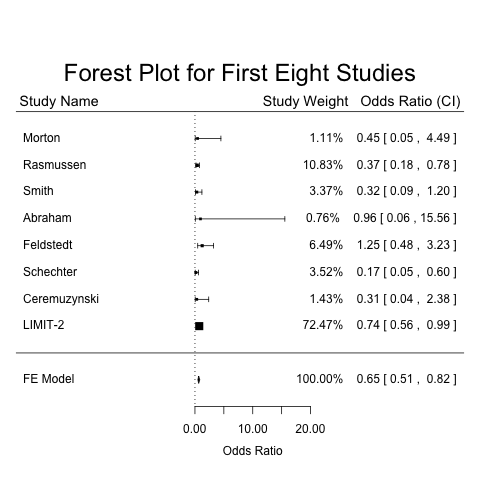
\includegraphics[scale=0.45]{./../figures/forest_early.png}
\\
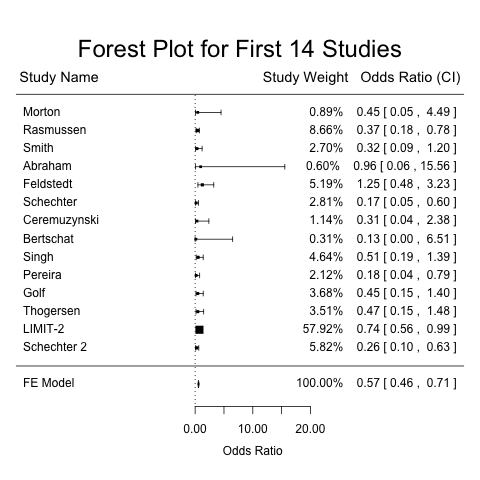
\includegraphics[scale=0.45]{./../figures/forest_middle.png}
\\
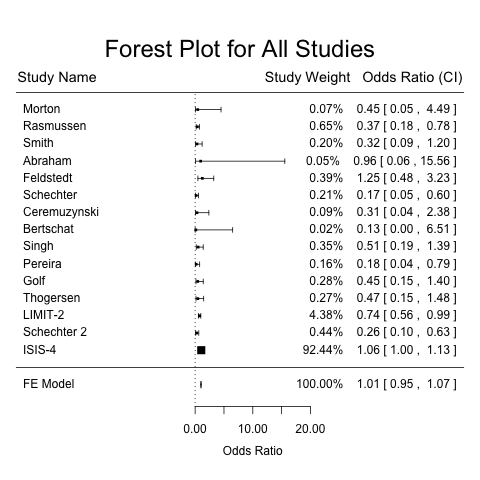
\includegraphics[scale=0.45]{./../figures/forest_late.png}
\label{fig:forests}
\caption{Forest plots showing the fixed-effect meta-analytic odds ratios for each trial set, plus the model weights assigned to each trial}
\end{figure}
\end{center}
Prior to interpreting the results shown in figure and table 2, recall:
\begin{itemize}
\item Odds ratios less than one indicate a beneficial effect (specifically, relatively lower odds of death for patients receiving magnesium following myocardial infarction than for patients receiving the control treatment).
\item Odds ratios higher than one indicate a harmful effect (specifically, relatively higher odds of death for patients receiving magnesium following myocardial infarction than for patients receiving the control treatment).
\end{itemize}

Now consider the forest plots shown in figure 1. First, note the fixed-effects model (fit using the Peto Method) was dominated by the trials with the largest sample sizes. For example, in the model fit using the first eight studies, the LIMIT-2 study received 72.47\% of the weight in the fixed-effects model. In the all-studies model, the ISIS-4 study received 92.44\% of the weight. This weighting causes the fixed-effects model odds ratio (OR) to change dramatically with the inclusion of the ISIS-4 trial in the trial set. Prior to the inclusion of the ISIS-4 model, the 14 study OR was 0.58 (with a 95\% CI of [0.46,0.71]). This indicates the odds of death for patients given magnesium following myocardial infarction was estimated to be 0.57 times the odds of death for control patients. This is clearly a dramatic effect (and one that would be extremely beneficial given the high prevalence of MI across the population). However, when the ISIS-4 trials is included, the fixed-effects OR estimate is 1.01 (with a 95\% CI of [0.0.95,1.07]). This indicates the absence of a statistically (or clinically) significant difference in the odds of death for patients in the treatment versus control groups.

In addition to the forest plots, a summary is presented in table \ref{tab:Table2}.  To interpret this table, we compare the estimated odds ratios and confidence intervals obtained for the fixed-effect and random-effects models. The primary observation is the insensitivity of the random-effects model to the ISIS-4 megastudy (relative to the fixed-effects model). This is expected, since random-effects model weights are less sensitive to sample size than fixed-effects model weights. As such, using the DerSimonian-Laird method, all the random-effects odd ratio estimates are significantly different than 1, and indicate a positive effect of Mg on death from complications due to myocardial infarction; for example, our final random-effects model (including ISIS-4) odds ratio estimate is 0.53 (95\% CI: [0.36, 0.77]), indicating patients receiving Mg have a 0.53 times odds of death compared to patients in the control group.

Overall, the random-effects model is preferable, since it relaxes the (potentially unfounded) assumption that the effect size is fixed across all trials. Note this assumption seems unfounded, especially given differences in study protocols (as noted in Higgins and Spiegelhalter's summary of criticims of the ISIS-4 megatrial) \cite{Original}. As such, the random-effects models seems to be a more accurate reflection of the underlying data generating process, and is preferable.

%------------------------------------------------

\section{Bayesian analysis}

Given the preference for the random-effects model (which places a distribution on the effect size), Bayesian modeling offers an opportunity to incorporate our prior beliefs about the effect size distribution (and potentially improve our model). Thus, we now turn to learning two different random-effects meta-analysis models. Our first model will use the reference prior $\delta \sim \textrm{N}(0, 10,000)$, while our second model will use the skeptical prior $\delta \sim \textrm{N}(0, 0.03)$
Note the reference prior is approximately uniform (since it is normal with very large variance), and the skeptical prior, adopted from Higgins and Spiegelhalter, is ``\emph{equivalent to a `trial' with 72 deaths in each group"} \cite{Original}.

Except for the differing priors on $\delta$, the two models are otherwise the same. Specifically, the model (equivalent to method (i) from Higgins and Spiegelhalter \cite{Original}) is the Bayesian version of the Peto method. For the $i^{\textrm{th}}$ study, we estimate the log odds ratio $Y_i \approx \delta_i$, and compute the variance $1/V_i$ of our estimate ($Y_i$). Following \cite{Original}, we define these estimates as
\begin{align*}
O_i &= r_i^M \\
E_i &= \frac{r_i^C + r_i^M}{n_i^C + n_i^M}n_i^M \\
V_i &= \frac{n_i^Cn_i^M(r_i^C + r_i^M)(n_i^C + n_i^M - r_i^C - r_i^M)}{(n_i^C + n_i^M)^2(n_i^C + n_i^M-1)} \\
Y_i &= \frac{O_i + E_i}{V_i} \sim \textrm{N}(\delta_i, 1/V_i)
\end{align*}
Next, with these estimates (and prior) in hand, our model is
\begin{align*}
\textrm{Reference prior on }\tau:&\qquad{} \textrm{Uniform}(0,100) \\
\textrm{Distribution of }\delta_i:&\qquad{} \textrm{N}(\delta,\tau^2) \\
\textrm{Distribution of }Y_i:&\qquad{} \textrm{N}(\delta_i,1/V_i)
\end{align*}
We find the posterior distributions for $\delta$ (for the sake of notation, going forward this will be referred to as the distribution of $\delta_{new}$) using 3 MCMC chains of 500,000 iterations each. First note convergence of the MCMC chains is apparent from the trace plots shown in figure \ref{fig:post_trace}. 
\begin{center}
\begin{figure}
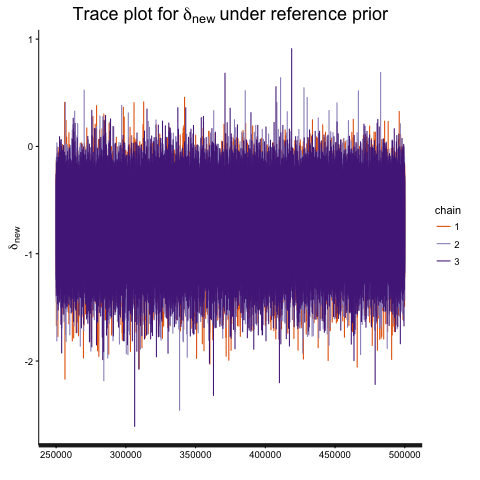
\includegraphics[scale=0.55]{./../figures/reference_trace.png}\\
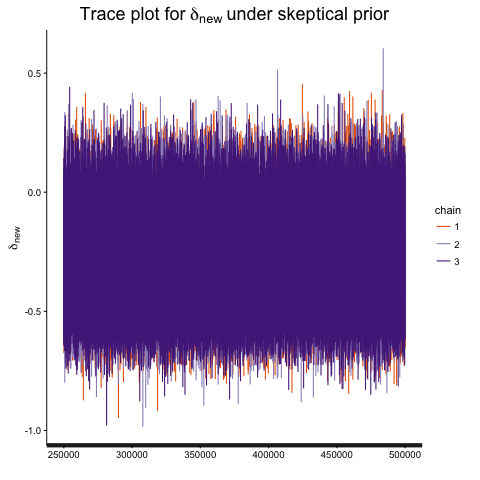
\includegraphics[scale=0.55]{./../figures/skeptical_trace.png}
\caption{Trace plots illustrating convergence of the MCMC chains}
\label{fig:post_trace}
\end{figure}
\end{center}
\begin{center}
\begin{figure}
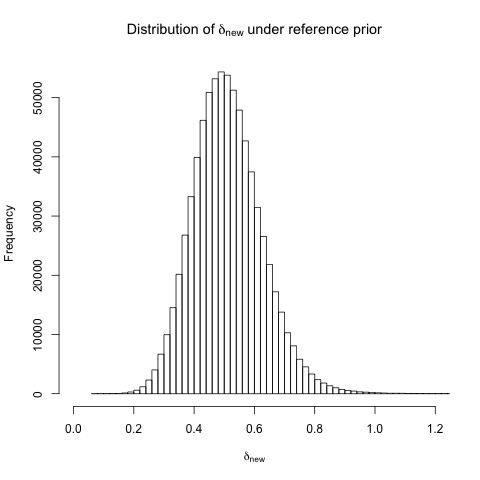
\includegraphics[scale=0.55]{./../figures/reference_hist.png}\\
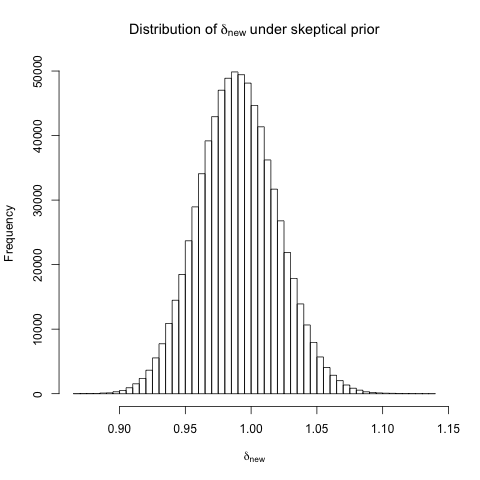
\includegraphics[scale=0.55]{./../figures/skeptical_hist.png}
\caption{Histograms showing the posterior distributions of $\delta_{new}$ under skeptical and reference priors. Note the $x$-axis scales are unequal; the posterior distribution has lower variance under the skeptical prior than under the reference prior}
\label{fig:post_hists}
\end{figure}
\end{center}
Next, having (visually) shown the convergence of the MCMC chains, the posterior distributions are presented as histograms in figure \ref{fig:post_hists}.



%------------------------------------------------

\section{Conclusion}

%----------------------------------------------------------------------------------------
%	REFERENCE LIST
%----------------------------------------------------------------------------------------

\bibliographystyle{unsrt}
\bibliography{sample}

%----------------------------------------------------------------------------------------

\end{document}